\section{İLETİM ORTAMLARI}
Temelde atmosfer ve kablo olmak üzere iki farklı iletim ortamı mevcuttur.Atmosfer rf(radyo frekans) dalgalarını kullanarak  iletişim gerçekleşir.
Kablolarda ise genellikle fiberoptik ve bakır kablo kullanılmaktadır.

\subsection{İKİ TELLİ BAKIR TELEFON HATTI }
Telefon iletişimini sağlamak için tasarlanmıştır.Temel band ve geniş band internet hizmeti verilmektedir.
Analog modülasyon teknikleryle en fazla 56 k b/s'lik band genişliği sağlar.xDSL teknolojileriyle 25 M b/s'lik band genişliğine ulaşmaktadır.  
%\begin{figure}[!ht]
  %  \includegraphics{images/ikitellibakırkablo}
  % \caption{İki telli Bakır Kablo}
  %  \label{fig:iki_telli_bakir_kablo}
 %\end{figure}

 \subsection{KOOKSİYEL(CCOKSİAL)KABLO}
 Genellikle elektiriksel gürültünün yoğun olduğu şartlarda kullanılırdı.Yalıtkan bir tüpün içerisinde  giden bir tel ve tüpün dışına sarılmış kafes şeklinde teller vardır.
 Yerel ağlarda (LAN) 180m'de(max) 10M b/s bant genişliği sağlar.Bu kullanımı 10 Base 2 olarak bilinir.Daha sonra 500 m mesafede çalıştırılacak hale getirilir. 10 Base 2 ismiyle standartlaştırılmıştır.50 ohm'luk direnç değeri vardır.
 BNC tarzında connectörler kullanılır.Günümüzde LAN'da hiç kullanılmamaktadır.Sebebi hem 1o M b/s  hızının çok düşük olması,hem de UTP kablolar kadar ekonomik ve işlevsel olmamasıdır.
 Bilgisayr ağlarında doğrusal (bus) topolojilerde kullanılmıştır. 
 %
  %\begin{figure}[!ht]
  %   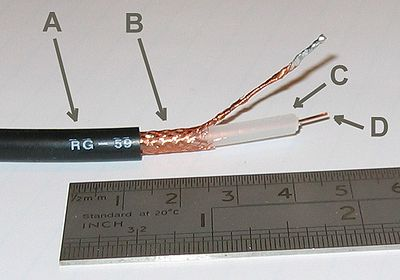
\includegraphics{images/400px-RG-59}
   % \caption{Kooksiyel Kablo}
    % \label{fig:kooksiyel_kablo}
  %\end{figure}


 \section*{AĞ TOPOLOJİLERİ }
%\begin{figure}[!ht]
%    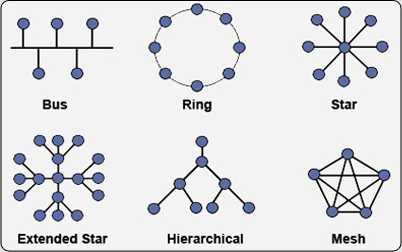
\includegraphics{../images/62_ağ_topolojisi.jpg}
%   \caption{Topolojiler}
%    \label{fig:topolojiler}
% \end{figure}
 % bu kısm notlarda yok topoloji nedir kısmını ben ekledim.
Ağ topolojileri nedir sorusunun en net cevabı, “bir ağı oluşturan cihazların fiziksel ve mantıksal yerleşimidir“.Network Topology (Ağ Topolojisi) Yerel Ağ Alanı (LAN) içerisinde bulunan bilgisayarların fiziksel ve mantıksal yerleşimini ifade eder. Fiziksel Topoloji ağ içerisinde bulunan tüm cihazların birbirlerine nasıl bağlanacağını ve bağlantı için ne tür kablo kullanacığını belirtirken Mantıksal Topoloji bu cihazların nasıl haberleşeceğini belirtir ve bu cihazları ortak bir protokol altında birleştirir. Kullanılmak istenen Ağ Teknolojisine göre farklı ağ topolojileri kullanılmaktadır.
Fiziksel Topolojinin 6 farklı çeşidi vardır. Bunlar Bus(Yol), Ring(Halka), Yıldız(Star), Ext Star(Gelişmiş Yıldız), Mesh(Örgü) ve Tree(Ağaç) topolojileridir. Broadcast(Yayın) ve Token Passing(İz) mantıksal topolojilere birer örnektir 

\subsection*{DOĞRUSAL (BUS) TOPOLOJİ}
Doğrusal bir hat üzerinde bilgisayarların T konnektörlerle bağlanması şeklinde kurulur.Hattın her iki ucunda 
sonlandırıcı kullanmak zorunludur.Kooksiyel kablo kullanılır.Ağın herhangi  bir noktasında arıza olması durumunda ağın tamamı çöker.Ağdaki veri trafiği tüm uçlara gider.
Herkes herkesin trafiğini görebilir.Bu yüzden çok fazla \textbf(çakışma(cooolision)) olur.
\begin{figure}[!ht]
    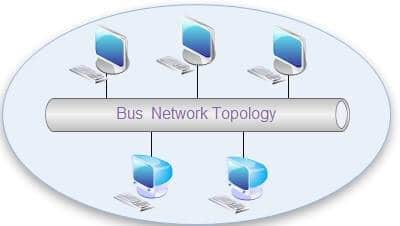
\includegraphics{images/bus-topolojisi}
   \caption{Bus Topolojisi}
   \label{fig:bustopolojisi}
 \end{figure}

\subsection*{HALKA (RING) TOPOLOJİ}
Doğrusal topolojiye benzer.Sonlandırıcı kullanılmaz.Hattın iki ucu birleşiktir.
Hatta sanal  bir jeton dolaşır(token).Jeton sırası gelen bilgisayar,jeton boş ise göndereceği veriyi hatta yerleştirir.
Bilgisayarlar sırayla  veri gönderdiklerinden çakışma daha azdır.Günümüzde hiç kullanılmamaktadır.
Herkes herkesin verisini kullanabilmektedir.
%bu fotoğraf en alta geçiyor düzeltilecek
%\begin{figure}[!ht]
%    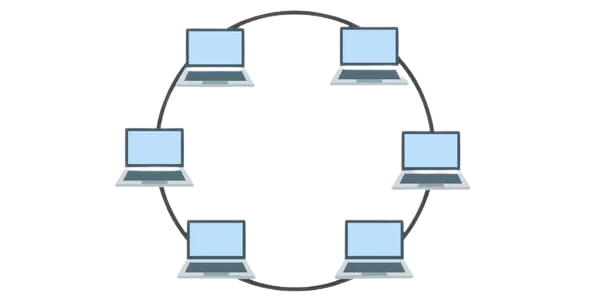
\includegraphics{images/ring-topology-removebg-preview}
%    \caption{Halka-Ring Topolojisi}
%   \label{fig:halka_topolojisi}
%  \end{figure}
%

\subsection*{YILDIZ (STAR) TOPOLOJİ}
Merkezde dağıtıcı bir cihaz olur.Burdan tüm bilgisayarlara birer kablo gider.Ağın bir noktasındaki arıza sadece ilgili bilgisayarın ağ bağlantısına zarar verir.Genellikle \textbf(bükümlü çift (twisted pair,xtp)) kullanılır.Trafiğin herkese mi gönderileceği ya da sadece ilgili ucamı gideceği dağıtıcıya bağlıdır.
Dağıtıcının  performansı ve kabiliyeti ağı doğrudan  etkiler.
Günümüzde en yaygın topolojidir.
%YERİ DÜZELTİLECEK
%\begin{figure}[!ht]
%    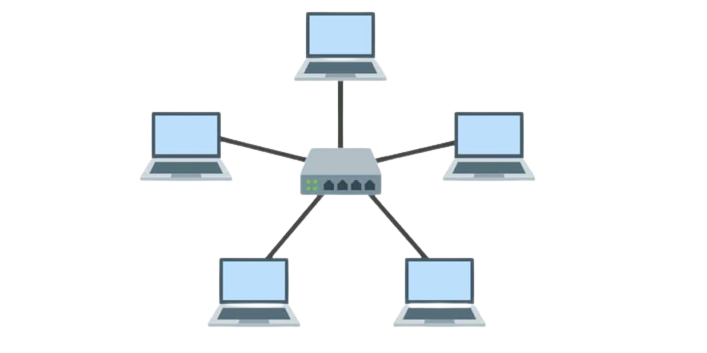
\includegraphics{images/star-Topology-1024x512-removebg-preview}
%    \caption{Yildiz-StarTopolojisi}
%   \label{fig:yildiz_topolojisi}
%  \end{figure}

\subsection*{ÖRGÜ (MESH)TOPOLOJİ}
%YERİ DÜZELTİLECEK
%\begin{figure}[!ht]
   % 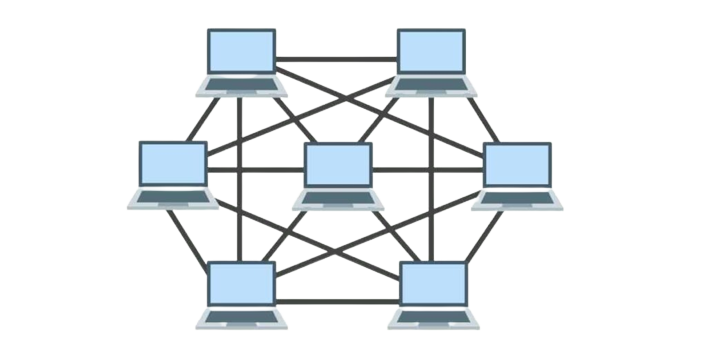
\includegraphics{images/mesh-topology-1-1024x512-removebg-preview}
    %\caption{Örgü-Mesh Topolojisi}
 %  \label{fig:Orgu_mesh_topolojisi}
  %\end{figure}
Uçları arasında birden fazla rota üzerinde haberleşme imkanı olan yapılardır.
Günümüzde genellikle farklı yıldız ağlar arasında yedekleme amacı olarak kullanılır.


\subsection{BÜKÜMLÜ ÇİFT KABLO}
  İçerisinde 4 çift bakır kablo bulunur.Kabloların birbireri üzerindeki direnç elektromanyetik etkisini azaltmak için ikişerli olarak sarılı durumundadırlar.
  Örneğin; UTP,CAT5,Ethernet Kablosu 
  %\begin{figure}[!ht]
  %  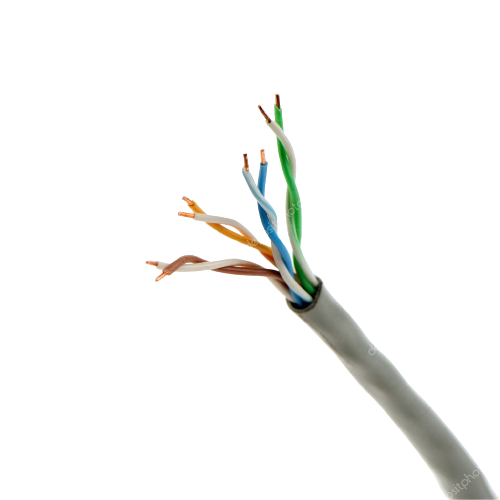
\includegraphics{images/bukumlukablo}
   % \caption{Bükümlü çift kablodan bir kesit}
 %\label{fig:Bukumlu_cift_kablo}
  %\end{figure}

\subsubsection{UTP(UNSHİLDED PWİSTED PAİR)Korumasız Bükümlü Çift} 
    8 iletkenin her biri ince bir yalıtkan ile kaplanmıştır.En dışında tamamını kaplayan bir yalıtkan vardır.
\subsubsection{STP(SHİLDED TWİSTED PAİR)} 
Her çiftin altında koruma (topraklama ) vardır.
\subsubsection{FTP(FOİLED TWİSTED PAİR )} 
4 çiftin tamamının etrafında folyo koruma vardır.
\subsubsection {S/FTP }
İkisinin de özelliğini taşımaktadır.
    
\subsection{FREKANSLARINA GÖRE BÜKÜMLÜ ÇİFT KABLO}
\textbf{CAT:}\\
\textbf{CAT1-CAT3} \\
Telefon hatlarında bulunur.\\
\textbf{CAT5} \\
En yaygın kullanılan ağ kablosudur.Azami 100 m mesafe ve 10 m b/s destekler\\
\textbf{CAT6} \\
100 m mesafede 1G b/s destekler.\\
\textit{10 BASE T} Ethernet(Eth)\\
\textit{100 BASE T} Fast Ethernet(Fa,Fe)\\
\textit{1000 BASE T} Gigabit Ethernet(G,GE)\\
Bükümlü çift CAT5 VE CAT6 Kabloları  sonlandırmak için RJ-45 adı verilen connektörler kullanılır.
Bu kablolar iki farklı iki şekilde sonlandırılabilir.\textbf{568-A,568-B}\\
Kablonun iki ucunun aynı standarlarla sonlandırılmasna \textbf{Düz(Straight kablo )} denir.İki ucunda iki farklı standartta sonlandırılma yapılırsa \textbf{çapraz(cross-over)kablo } adı verilir.